\section{Results}\label{sec:results}

\subsection{Model fit}

The production model reaches a test AUC between 0.863 and 0.869 across the five replicates, against 0.865 to 0.870 for the true log odds, and a test log loss between 0.200 and 0.209, against 0.198 to 0.208. Aggregate measures of this kind do not show how accurate the model is for an individual applicant, so the fitted log odds were compared with the true log odds directly. The root mean squared error is between 0.20 and 0.23 on the test sample and between 0.23 and 0.30 for the declined applicants. It is largest in the highest decile of true risk (0.33 to 0.40). On the hybrid records evaluated by the attribution game, which combine blocks of a declined applicant and a passing reference, the error is between 0.24 and 0.27 and its 95th percentile is between 0.47 and 0.53. These errors are small relative to the mean score gap of 1.48 but not negligible for individual blocks, which matters for the comparisons of attribution with the true model below. The passing band contains between 2{,}199 and 2{,}564 reference records.

The full model and outcome-fitted reduced models use Platt recalibration; the soft-target projection regressions are not separately recalibrated. Leaf-local probabilities come from smoothed class frequencies. On the simulation test samples, the full-model calibration slopes after recalibration range from 0.97 to 1.02. This supports the probability scale used in the comparison but does not eliminate the individual log-odds errors above. Appendix~\ref{app:calibration} gives the full calibration results.




\begin{table}[t]\centering\small
\caption{Grouped baseline-Shapley attribution of the score gap for 400 declined applicants per replicate, means over five replicates. Attributions are in estimated default log odds; the mean total gap to the references is 1.48. Leading-reason shares are the fractions of applicants whose largest attribution falls on each block.}
\label{tab:aarc}
\resizebox{\linewidth}{!}{\begin{tabular}{@{}lrrrrrr@{}}\toprule
& Revolving & Delinq. & File age & Seeking & Install. & Public rec.\\\midrule
Mean attribution, production model, score band & 0.42 & 0.85 & $-$0.02 & 0.15 & 0.03 & 0.05\\
Mean attribution, true log odds, score band & 0.40 & 0.86 & $-$0.03 & 0.16 & 0.04 & 0.05\\
Mean attribution, production model, proximity & 0.46 & 0.74 & 0.03 & 0.15 & 0.03 & 0.06\\\midrule
Leading-reason share, production model & 0.26 & 0.57 & 0.05 & 0.07 & 0.00 & 0.06\\
Leading-reason share, true log odds & 0.23 & 0.56 & 0.06 & 0.08 & 0.00 & 0.07\\
Leading-reason share, proximity references & 0.33 & 0.51 & 0.01 & 0.09 & 0.01 & 0.05\\
\bottomrule\end{tabular}}
\end{table}


\subsection{Attribution against passing references}\label{sec:case}

Delinquency and revolving credit lead the score attribution for 57 and 26 percent of simulated declines, respectively. The average applicant-reference gap is 1.48 log-odds units. The fitted and true-model attributions against the same references have the same leading block for 93.2 percent of applicants (91.8--94.2 percent across replicates), and their two leading blocks overlap in 94.4 percent of positions. These comparisons isolate model fit while holding the reference records fixed (Table~\ref{tab:aarc}).

The reference policy has a larger effect than the difference between the fitted and true models. Replacing the score-band references by the most leaf-proximate references in the band changes the leading block for 32 percent of applicants, with a median Spearman correlation of 0.67 between the two attribution vectors. The most frequent changes are from delinquency to revolving credit (11 percent of applicants) and from revolving credit to delinquency (5 percent). For the applicants whose leading block changes from delinquency to revolving credit, about 45 per replicate, the proximity references have more delinquency than the score-band references (on average 1.02 against 0.61 accounts 30 or more days past due and 0.24 against 0.05 accounts 90 or more days past due) and lower utilization (0.38 against 0.53). These applicants average 1.22 delinquent accounts and utilization of 0.59. Proximity references are therefore closer to these applicants in delinquency and farther from them in utilization, which is consistent with the shift of the leading block from delinquency to revolving credit.

\begin{table}[t]\centering\small
\caption{A declined applicant from replicate 1 whose leading block changes with the reference policy. Reference columns give means over the 50 references of each policy; the share of references with any account 30+ days past due is 0.54 under the score-band policy and 1.00 under the proximity policy. The lower panel gives block attributions $C^f_j$ of the production model and the applicant's oracle evidence $W_j$ and $E_j$ (logit units).}
\label{tab:case}
\begin{tabular}{@{}lrrr@{}}\toprule
& Applicant & Score-band references & Proximity references\\\midrule
Revolving utilization & 0.53 & 0.53 & 0.27\\
Revolving limit (\$) & 30{,}809 & 15{,}936 & 29{,}493\\
Revolving balance (\$) & 16{,}229 & 8{,}176 & 8{,}089\\
Accounts 30+ days past due & 1.00 & 0.58 & 1.00\\
Accounts 60+ days past due & 1.00 & 0.20 & 0.84\\
Accounts 90+ days past due & 1.00 & 0.10 & 0.40\\
Oldest trade (months) & 294 & 81 & 181\\
Inquiries in 6 months & 1.00 & 1.98 & 1.02\\
Installment fraction outstanding & 0.36 & 0.59 & 0.43\\
Public record & 0.00 & 0.14 & 0.00\\
\midrule & Attribution, score band & Attribution, proximity & Oracle $W_j$ / $E_j$\\\midrule
Revolving & $-$0.07 & +1.14 & +1.05 / +0.71\\
Delinquency & +1.87 & +0.61 & +2.01 / +1.96\\
File age & +0.40 & 0.00 & +0.04 / $-$0.19\\
Credit seeking & $-$0.18 & +0.02 & $-$0.15 / $-$0.23\\
Installment & $-$0.13 & $-$0.01 & $-$0.17 / $-$0.56\\
Public record & $-$0.13 & 0.00 & $-$0.04 / $-$0.05\\
Total gap & 1.76 & 1.75 & \\
\bottomrule\end{tabular}
\end{table}


The applicant in Table~\ref{tab:case} has one account 90 or more days past due, with the most recent delinquency one month earlier, and uses 53 percent of a revolving limit of \$30{,}809. Against score-band references, delinquency contributes 1.87 log-odds units to a total gap of 1.76. A contribution can exceed the gap because favorable contributions from other blocks offset it. Revolving credit contributes $-0.07$ against these references, whose mean utilization is also 53 percent and among whom 54 percent have any delinquency.

Every proximity reference has a delinquency, including 40 percent with an account 90 or more days past due. The delinquency contribution falls to 0.61. These references have mean utilization of 27 percent and a mean limit of \$29{,}493; revolving credit becomes the largest contribution at 1.14. The applicant's balance is about twice their mean balance at a similar mean limit, pointing to utilization as a candidate description. A grouped allocation does not separate utilization, balance and limit, however, and a field-level conclusion would need to preserve their defining identity.

The case was selected for the largest change in the revolving-minus-delinquency attribution among the relevant transitions, so it illustrates a pronounced rather than typical change. Its oracle conditional evidence is adverse for both revolving credit (1.05) and delinquency (2.01). Choosing which of the two passing populations is appropriate remains a reference-policy decision; the attribution accounts for the score contrast once that decision has been made.

The applicant's oldest trade is 294 months, yet file age contributes $+0.40$ against score-band references and approximately zero against proximity references. In this deliberately constructed risk model, younger files receive lower risk at high utilization. For a reference $r$, the true-model file-age allocation is $\{\tau(x)-\tau(r)\}\{0.6-1.7(u(x)+u(r))\}$, obtained by averaging whether file age enters before or after revolving credit. Averaging over the saved references gives 0.460 and 0.005 logit units, respectively, matching the exact true-model allocations. The positive fitted contribution against the score band therefore follows the constructed interaction; it is not evidence that a long credit history is generally adverse.


The distinction also appears in the averages. Mean revolving attribution is 0.42, close to coalition evidence of 0.43 but above last-entry evidence of 0.19. Delinquency attribution is 0.85, compared with coalition evidence of 0.62. The score-band references have more delinquency than the population average (0.62 versus 0.38 accounts 30 or more days past due), so a simple ``cleaner references'' explanation does not account for that difference; its mechanism has not been isolated. The installment attribution of 0.03 is much smaller than coalition evidence of 0.12, consistent with the counterfactual finding that most of its order-averaged evidence remains when the direct installment term is removed. Figure~\ref{fig:attr} separates the fitted-score comparisons from the population evidence allocations.

\begin{figure}[t]
\centering
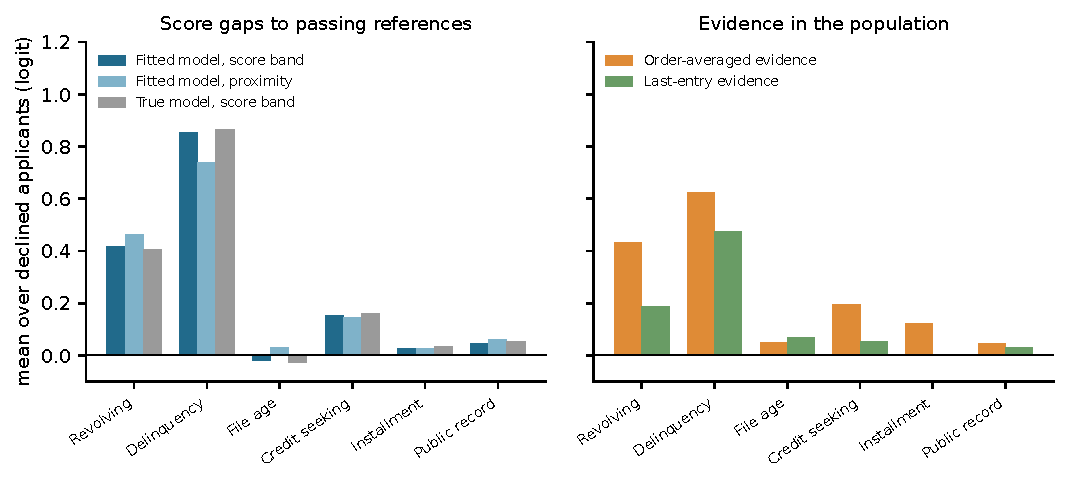
\includegraphics[width=\linewidth]{figures/attribution_vs_evidence.pdf}
\caption{Mean attribution of the score gap and mean oracle evidence by block for the declined applicants, averaged over five replicates. Left: score attributions against the specified passing references. Right: population evidence allocated by order averaging or measured after all other blocks are known. The panels share units but use different comparison distributions.}
\label{fig:attr}
\end{figure}



The reference-based evidence comparison of Proposition~\ref{prop:collapse} was computed with the direct estimator for every declined applicant, block and reference. The largest observed difference from the single-block swap on the production model is $7.2\times10^{-7}$, consistent with single-precision rounding of the model outputs, so the block-excluded models do not contribute to the comparison.


\subsection{Accuracy of the direct and projection estimators}

Revolving credit and delinquency provide the clearest evidence-recovery test. Their oracle evidence varies substantially across applicants, and projection recovers its sign for 99 to 100 percent of records with absolute evidence above 0.25. Across all blocks, projection has lower RMSE than separate refits: 0.09--0.18 versus 0.15--0.21 logit units (Table~\ref{tab:accuracy}). For revolving credit and delinquency, the oracle standard deviations are 0.51 and 0.78, respectively, against projection errors of 0.17 and 0.18.

Small conditional effects are harder to recover. Installment evidence has oracle standard deviation 0.10, and only 1 percent of applicants have absolute evidence above 0.25. Projection and direct estimates have correlations of 0.74 and 0.55 with the oracle. Their errors must therefore be judged against a small signal, not simply against the larger errors of marginal WoE. The zero-evidence rows of Table~\ref{tab:accuracy} make this comparison explicit.

The estimators share a full model but obtain their reduced probabilities differently: the direct method learns from binary outcomes, whereas projection learns from the full model's probabilities. Equation~\eqref{eq:error_difference} shows why the evidence error depends on both reduced-model accuracy and cancellation of shared errors. The saved predictions allow those terms to be assessed directly.

Projection improves both components of the evidence comparison. For file age, reduced-posterior RMSE falls from 0.218 to 0.190, while correlation of full and reduced errors rises from 0.625 to 0.793. For installment debt, reduced-posterior RMSE changes only from 0.211 to 0.202, but the error correlation rises from 0.738 to 0.902. The cross-product decomposition in Appendix~\ref{app:errors} confirms that greater cancellation contributes to the smaller evidence error. An accurate difference therefore does not imply equally accurate full and reduced risk estimates.

The combined evaluation sample contains 28.3 percent current-model declines, rather than the 20 percent targeted by the policy. Table~\ref{tab:decline_accuracy} reports errors separately for the 400 sampled declines per replicate. Errors are larger among declines for every block, although projection retains lower error than direct refitting.


File age illustrates what the marginal transformation misses in this constructed population. Among applicants with utilization above 50 percent, the oracle file-age evidence averages $-0.45$ for files younger than 48 months and $+0.25$ for established files. Projection gives $-0.41$ and $+0.23$, whereas global WoE averages $+0.08$ and $0.00$ for the corresponding classes. Across records with material class-level file-age evidence, global WoE has the oracle sign in only 28 percent of cases. The generating model deliberately makes younger files less adverse at high utilization: $\partial f^\ast/\partial\tau=0.6-3.4u$. Conditional evidence also depends on where the observed file age lies in its distribution given the other blocks. These group means demonstrate recovery of a designed interaction, not a claim that young credit files are generally favorable in lending.

For revolving credit, Figure~\ref{fig:revolving} shows increasing evidence with utilization among established files and a much flatter pattern among young files. Each point is a different applicant, so its vertical position also reflects the other characteristics. The low-utilization comparison illustrates the distinction between marginal and conditional evidence: global WoE averages $-1.71$ for the class with utilization below 20 percent in both file-age groups, while oracle revolving evidence averages $-0.49$ for established files and $-0.12$ for young files. Low utilization conveys information about financial stress that delinquency and inquiries can already supply.

\begin{figure}[t]
\centering
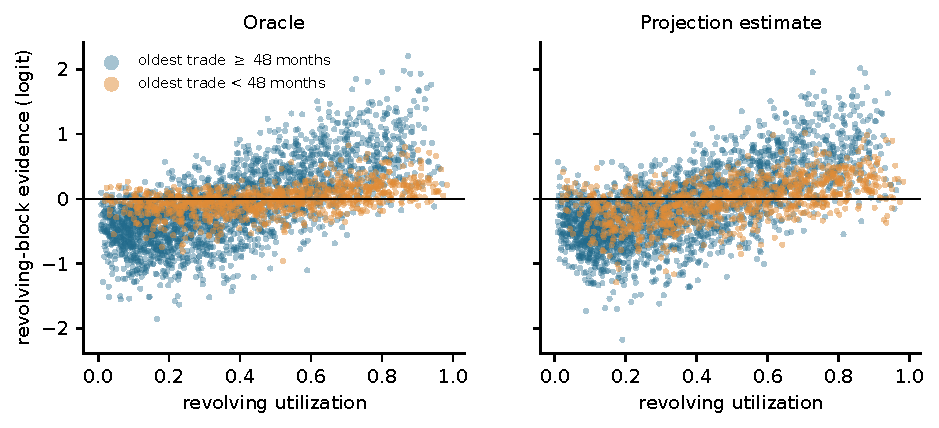
\includegraphics[width=\linewidth]{figures/revolving_evidence.pdf}
\caption{Revolving-block conditional evidence for evaluation applicants in replicate 1. Each point is an applicant with its own remaining credit characteristics. Oracle evidence (left) varies less with utilization in the under-48-month group; projection (right) recovers the broad difference between groups with additional dispersion. Zero marks no change in default odds from observing the revolving block. These are cross-applicant patterns, not effects holding the remaining fields fixed.}
\label{fig:revolving}
\end{figure}

\begin{table}[t]\centering\small
\caption{Error of conditional evidence estimates against the oracle in the bureau-style simulation: root mean squared error (logit units), mean over five replicates, for about 3{,}350 combined evaluation applicants per replicate. Direct and projection estimates are compared with the pointwise evidence $W_j$ and the global and leaf-local estimates with the class-level evidence $W^B_j$; errors in different panels refer to different targets and are not compared with each other. The first two rows give the standard deviation of the oracle across applicants. Zero-evidence baselines assign zero to every applicant for each target. Replicate standard deviations of the RMSE are at most 0.02 for direct and projection estimates and at most 0.07 for leaf-local estimates.}
\label{tab:accuracy}
\resizebox{\linewidth}{!}{\begin{tabular}{@{}lrrrrrr@{}}\toprule
& Revolving & Delinq. & File age & Seeking & Install. & Public rec.\\\midrule
Oracle sd, pointwise $W_j$ & 0.51 & 0.78 & 0.31 & 0.29 & 0.10 & 0.20\\
Oracle sd, class-level $W^B_j$ & 0.46 & 0.68 & 0.29 & 0.26 & 0.09 & 0.20\\\midrule
Zero evidence, pointwise target & 0.51 & 0.79 & 0.31 & 0.29 & 0.10 & 0.20\\
Direct & 0.20 & 0.21 & 0.19 & 0.17 & 0.15 & 0.16\\
Projection & 0.17 & 0.18 & 0.13 & 0.13 & 0.09 & 0.10\\\midrule
Zero evidence, class-level target & 0.47 & 0.69 & 0.29 & 0.26 & 0.09 & 0.20\\
Global WoE of class & 0.97 & 0.59 & 0.38 & 0.63 & 0.78 & 0.12\\
Leaf-local, default geometry, $\kappa=1$ & 0.72 & 0.42 & 0.33 & 0.46 & 0.61 & 0.10\\
Leaf-local, default geometry, selected $\kappa$ & 0.27 & 0.16 & 0.28 & 0.19 & 0.23 & 0.07\\
Leaf-local, class geometry, $\kappa=1$ & 0.71 & 0.42 & 0.33 & 0.40 & 0.53 & 0.08\\
Leaf-local, class geometry, selected $\kappa$ & 0.24 & 0.16 & 0.22 & 0.14 & 0.18 & 0.05\\
\midrule
Sign agreement$^{a}$, projection & 0.99 & 1.00 & 0.99 & 0.99 & 0.96 & 1.00\\
Sign agreement, global WoE & 0.90 & 0.96 & 0.28 & 0.97 & -- & 1.00\\
Sign agreement, leaf-local (class, selected) & 0.99 & 1.00 & 0.94 & 0.99 & -- & 1.00\\
Share with $|W_j|>0.25$ & 0.55 & 0.76 & 0.24 & 0.37 & 0.01 & 0.05\\
\bottomrule\end{tabular}}
\par\smallskip\raggedright\footnotesize $^{a}$Share of applicants with $|$oracle$|>0.25$ whose estimate has the oracle's sign; -- indicates 20 or fewer such applicants. The qualifying records can differ between the two targets.
\end{table}



\subsection{Accuracy of the leaf-local estimator}

The leaf-local estimator targets the class-level evidence $W^B_j$, which differs from the pointwise evidence by an RMSE of 0.21 for revolving credit and 0.40 for delinquency because the block classes are coarse. Its errors are therefore compared with those of global WoE, the marginal class-level WoE used as a baseline and evaluated against the same conditional class-level oracle, and not with the pointwise estimators. With the proximity kernel of Eq.~\eqref{eq:kernel} used as originally specified ($\kappa=1$), the estimator improves on global WoE for every block, but its error remains larger than the oracle standard deviation for the revolving, file-age, credit-seeking and installment blocks (Table~\ref{tab:accuracy}). The effective sample sizes indicate how broadly the records are weighted. With $\kappa=1$, the median default-class effective sample size is between 5{,}992 and 7{,}133 in an evidence sample containing about 8{,}700 defaults, so the weights spread over most of the sample and the estimate stays close to the global value. Each root-to-leaf path of a depth-4 tree has at most four splits, and averaging leaf membership over trees does not restrict all the other fields at once.

Raising the kernel to a power concentrates the weights (Figure~\ref{fig:kernel}). The held-out likelihood criterion selected $\kappa=8$ in 22 of the 30 block-replicate combinations for the default geometry, $\kappa=4$ in 6 and $\kappa=16$ in 2, and selected the smallest smoothing constant, $\lambda=0.1$, in 27 of 30. The oracle error is lowest at $\kappa=8$ for four blocks and at $\kappa=4$ for the other two, so the criterion, which uses no oracle information, selects at or next to the best exponent. At the selected exponent, the median default-class effective sample size falls to between 110 and 814 and the error falls by a factor of 1.2 (file age) to 2.7 (revolving credit) relative to $\kappa=1$. Larger exponents increase the error again as the effective sample size of defaulters becomes small. Within a block, the error decreases with the local effective sample size: for revolving credit, the RMSE is 0.32 in the lowest tercile of default-class effective sample size and 0.23 in the highest.

At the selected exponent, class-prediction neighborhoods have lower error than default-prediction neighborhoods for every block, most noticeably file age (0.22 versus 0.28) and installment debt (0.18 versus 0.23). The class geometry better recovers the held-out class frequencies in this experiment. Yet the installment error of 0.18 remains larger than the 0.095 RMSE obtained by assigning zero class-level evidence to every applicant. H2 is supported as an improvement over marginal WoE, particularly with concentrated weights; that improvement does not establish accurate recovery of every block's conditional evidence.

Table~\ref{tab:samplesize} repeats the class-geometry estimate for replicate 1 with smaller evidence samples drawn from the same population. The error rises as the sample shrinks, from 0.22 to 0.62 for revolving credit and from 0.16 to 0.63 for installment between 100{,}000 and 2{,}500 records. Even with 2{,}500 records the estimate has lower error than the global WoE for every block. The experiment varies only the evidence sample; the geometry models and the calibration records are unchanged.

\begin{figure}[t]
\centering
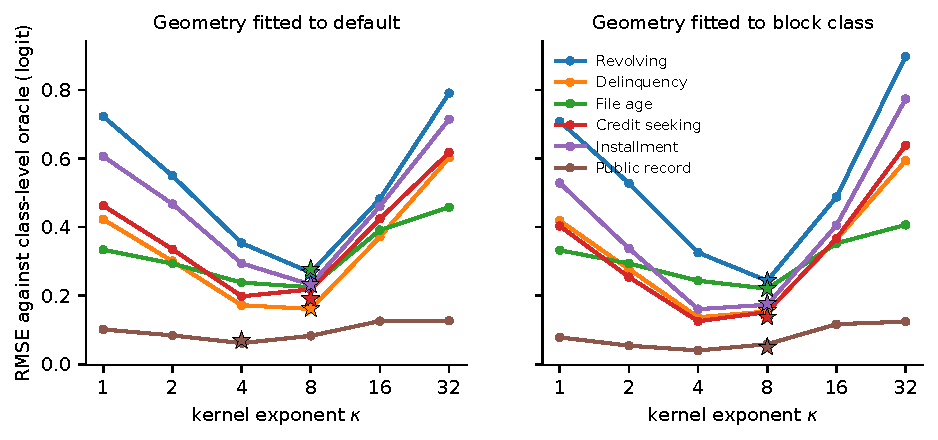
\includegraphics[width=\linewidth]{figures/kernel_exponent.pdf}
\caption{Leaf-local RMSE against the class-level oracle across kernel exponents. Lines minimize oracle error over the smoothing constant after averaging across replicates; they describe the error surface rather than a deployable selection rule. Stars show mean RMSE at the held-out-likelihood-selected exponent and smoothing constant, placed at the modal selected exponent for each block. $\kappa=1$ is the unsharpened proximity average.}
\label{fig:kernel}
\end{figure}

\begin{table}[t]\centering\small
\caption{Leaf-local estimation with evidence samples of different sizes, replicate 1. RMSE against the class-level oracle for the class geometry at the selected $(\kappa,\lambda)$, and for global WoE computed from the same subsample. The last row gives the median default-class effective sample size at 100{,}000 records.}
\label{tab:samplesize}
\resizebox{\linewidth}{!}{\begin{tabular}{@{}lrrrrrr@{}}\toprule
Evidence records & Revolving & Delinq. & File age & Seeking & Install. & Public rec.\\\midrule
2{,}500 & 0.62 & 0.32 & 0.41 & 0.36 & 0.63 & 0.06\\
10{,}000 & 0.51 & 0.19 & 0.39 & 0.22 & 0.32 & 0.07\\
30{,}000 & 0.36 & 0.17 & 0.29 & 0.16 & 0.20 & 0.11\\
100{,}000 & 0.22 & 0.14 & 0.23 & 0.15 & 0.16 & 0.08\\
Global WoE, 100{,}000 & 0.92 & 0.58 & 0.39 & 0.62 & 0.77 & 0.13\\
Global WoE, 2{,}500 & 1.01 & 0.66 & 0.45 & 0.71 & 0.98 & 0.14\\
Default-class ESS, 100{,}000 & 170 & 171 & 357 & 271 & 1061 & 271\\
\bottomrule\end{tabular}}
\end{table}



\subsection{Additivity and coalition evidence}

The leave-one-block-out values leave much of the total evidence unallocated for most declined applicants. Their mean sum is 0.74--0.88 across replicates, compared with total evidence of 1.39--1.58. The sum falls below the total by more than 0.05 for 75--81 percent of applicants and exceeds it by more than 0.05 for 15--21 percent. These are signs of an allocation discrepancy, not counts of redundant and synergistic applicants. Between 1 and 3 percent of model declines have negative population evidence, so decline status alone does not imply risk above the population average.

Order averaging allocates the total and yields projection errors of 0.05--0.18 for $E_j$, against oracle standard deviations of 0.28--1.14 (Table~\ref{tab:coalition}). The mean excess over last-entry evidence is largest for revolving credit (0.24), delinquency (0.15), credit seeking (0.14) and installment debt (0.12), and slightly negative for file age. The installment counterfactual allows a more specific interpretation than these signed averages alone.

The installment block illustrates the difference between applicant-level and order-averaged evidence. Over the test applicants, its leave-one-block-out evidence has standard deviation 0.10 and mean absolute value 0.08, and over the declined applicants its mean is 0.00 with standard deviation 0.09: the direct term $0.8\times\text{fraction}$ in Eq.~\eqref{eq:truth} produces evidence of both signs that averages out. To separate the direct term from the association of the installment fraction with financial stress, the oracle was recomputed for 1{,}000 test applicants and 200 declined applicants of replicate 1 with the direct term removed. The leave-one-block-out evidence of the installment block is then exactly zero, while its mean coalition evidence for the declined applicants falls only from 0.129 to 0.116. Most of the block's average coalition evidence for these applicants therefore comes from its association with the other blocks, and its applicant-level conditional evidence comes from the direct term.

\begin{table}[t]\centering\small
\caption{Coalition evidence of the 400 declined applicants per replicate and the effect of the earlier approval policy, means over five replicates (logit units). The coalition excess is $H_j=E_j-W_j$. The absolute booked-minus-through-the-door difference $|W^b_j-W_j|$ is computed from the oracle for the test applicants; earlier-policy declines are applicants with booking probability $s(x)<0.5$ and current-model declines are applicants with $f(x)>c$. The last three rows give the RMSE of direct estimates fitted on booked accounts only, against the through-the-door and booked oracles, and of direct estimates fitted on all applicants against the through-the-door oracle.}
\label{tab:coalition}
\resizebox{\linewidth}{!}{\begin{tabular}{@{}lrrrrrr@{}}\toprule
& Revolving & Delinq. & File age & Seeking & Install. & Public rec.\\\midrule
Coalition evidence $E_j$, oracle mean & 0.43 & 0.62 & 0.05 & 0.19 & 0.12 & 0.05\\
Leave-one-block-out $W_j$, oracle mean & 0.19 & 0.47 & 0.07 & 0.05 & 0.00 & 0.03\\
Coalition excess $H_j$, oracle mean & 0.24 & 0.15 & $-$0.02 & 0.14 & 0.12 & 0.01\\
RMSE of projection estimate of $E_j$ & 0.09 & 0.18 & 0.07 & 0.08 & 0.05 & 0.06\\
Oracle sd of $E_j$ & 0.68 & 1.14 & 0.28 & 0.57 & 0.35 & 0.35\\\midrule
$|W^b_j-W_j|$, all test applicants & 0.23 & 0.35 & 0.00 & 0.08 & 0.00 & 0.05\\
$|W^b_j-W_j|$, earlier-policy declines & 0.47 & 0.75 & 0.00 & 0.21 & 0.00 & 0.09\\
$|W^b_j-W_j|$, current-model declines & 0.54 & 0.74 & 0.00 & 0.22 & 0.00 & 0.09\\
Direct, booked fit vs.\ through-the-door oracle & 0.40 & 0.50 & 0.27 & 0.26 & 0.22 & 0.25\\
Direct, booked fit vs.\ booked oracle & 0.31 & 0.40 & 0.27 & 0.26 & 0.22 & 0.26\\
Direct, all-applicant fit vs.\ through-the-door oracle & 0.20 & 0.21 & 0.19 & 0.17 & 0.15 & 0.16\\
\bottomrule\end{tabular}}
\end{table}



\subsection{Booked-population evidence}

Booking changes the comparison distribution for revolving credit, delinquency, credit seeking and public records, the four blocks used by the earlier policy. Their mean booked-minus-through-the-door evidence differences are positive. For revolving credit and delinquency they average 0.23 and 0.35 over the evaluation sample, rising to 0.54 and 0.74 among current-model declines (Table~\ref{tab:coalition}). Among applicants with earlier-policy booking probability below 0.5, the corresponding means are 0.47 and 0.75. The two decline groups overlap substantially: 93 percent of current-model declines also have booking probability below 0.5.

File age and installment debt are absent from that policy, so their population evidence differences are zero up to numerical error. The sign for the policy's blocks is an empirical average, not a universal consequence of the booking rule: 11 revolving estimates across five replicates are slightly negative, with minimum $-0.0008$. The conditional covariance condition of Proposition~\ref{prop:selection} was not verified, and the model's utilization effect is not monotone for the youngest files.

Direct estimates fitted on booked accounts are closer to the booked oracle than to the through-the-door oracle: revolving RMSE is 0.31 versus 0.40, and delinquency RMSE is 0.40 versus 0.50. They also have larger error than all-applicant fits for blocks unaffected by population selection. The smaller booked sample and its 3.3 percent default rate accompany that loss of accuracy. The main selection finding is that booked-population evidence represents a different conditional comparison, especially for applicants classified as declines.


\subsection{FICO HELOC data}

The HELOC model has test AUC 0.782--0.807 across splits. Its fitted Platt slope ranges from 0.81 to 1.18; test calibration slopes range from 0.87 to 1.14 and intercepts from $-0.19$ to $0.08$. The raw margins have slopes of 0.91--1.08, and one recalibration moves a test slope from 0.91 to 0.87. These ranges describe small-sample calibration uncertainty rather than evidence that recalibration uniformly improves the predictions. The calibration sample contains about 940 records, and the evidence sample about 2{,}360. Passing bands contain 45--76 references.

Direct and projection evidence are correlated most strongly for delinquency (0.84) and revolving burden (0.87), with inquiry correlation 0.76. Agreement is weaker for trade volume (0.50) and installment burden (0.35), the two blocks with the least estimated evidence (Table~\ref{tab:heloc}). These methods share the full model, so their agreement is not an independent accuracy check.

The leaf-local estimates correlate with global WoE at 0.69 to 0.95 for five of six blocks and with the projection estimates at 0.04 to 0.76. The class-balanced criterion selected $\kappa=4$ in 44 of the 60 block-split combinations, $\kappa=8$ in 11 and $\kappa=2$ in 5, and $\lambda=0.1$ in 54. At these settings the median default-class kernel-weighted count is between 7 and 26 and the median default-class effective sample size between 88 and 251. The mean absolute difference between the leaf-local estimate and the global WoE of the class is between 0.13 and 0.28, against standard deviations of the global WoE across applicants of 0.18 to 0.81. The leaf-local estimates therefore depart from global WoE, but without an oracle it cannot be determined whether the departures are accurate, and the low correlation with the projection estimates for trade volume and installment burden is unexplained. The simulation shows that 2{,}500 evidence records can be enough for the leaf-local estimator to improve on global WoE in that population. It does not establish a sample-size requirement for HELOC, and the HELOC results provide limited evidence about leaf-local estimation in the configuration studied.

The estimated leave-one-block-out evidence sums to less than the estimated total evidence for 45 to 61 percent of declined applicants and to more for 36 to 50 percent. The estimated coalition excess is small for every block. For delinquency and revolving burden, which together lead for 71 percent of declined applicants, the mean attribution (0.37 and 0.36) is close to both the coalition evidence (0.30 and 0.37) and the leave-one-block-out evidence (0.30 and 0.33).

\begin{table}[t]\centering\small
\caption{FICO HELOC data, ten random splits. Correlations are across test applicants within a split, averaged over splits. Means of $E_j$, $W_j$ and the attribution $C^f_j$ are over declined applicants. Estimated evidence uses the projection estimator.}
\label{tab:heloc}
\resizebox{\linewidth}{!}{\begin{tabular}{@{}lrrrrrr@{}}\toprule
& Delinq. & File age & Trades & Inquiries & Revolving & Install.\\\midrule
Corr(direct, projection) & 0.84 & 0.72 & 0.50 & 0.76 & 0.87 & 0.35\\
Corr(projection, leaf-local default geometry) & 0.75 & 0.58 & 0.14 & 0.48 & 0.76 & 0.04\\
Corr(leaf-local default geometry, global WoE) & 0.93 & 0.89 & 0.69 & 0.92 & 0.95 & 0.46\\\midrule
Mean coalition evidence $E_j$ & 0.30 & 0.15 & 0.09 & 0.13 & 0.37 & 0.02\\
Mean leave-one-block-out $W_j$ & 0.30 & 0.14 & 0.04 & 0.13 & 0.33 & 0.04\\
Mean attribution $C^f_j$ & 0.37 & 0.22 & 0.11 & 0.18 & 0.36 & 0.01\\
Leading-reason share & 0.39 & 0.20 & 0.04 & 0.06 & 0.32 & 0.00\\
\bottomrule\end{tabular}}
\end{table}

